\documentclass[../main.tex]{subfiles}

\begin{document}
\label{apendice_ecuaciones_2}


En este apéndice se tratará la resolución de las ecuaciones diferenciales que nos darán como resultado las ecuaciones que modelan el circuito RL y que posteriormente, serán utilizadas en la implementación de dicha simulación.

\subsection{Constitución de corriente en un circuito RL}

\begin{figure}[!h]
    \centering
    \subfloat[Instante inicial. Intensidad nula.]{
        \label{fig::circuito_rl_1_2 }
        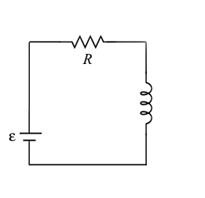
\includegraphics[width=0.33\textwidth]{images/Circuito_RL.png}
    }
    \subfloat[Autoinducción de corriente (carga)]{
        \label{fig::circuito_rl_2_2}
        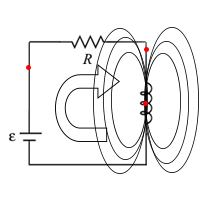
\includegraphics[width=0.33\textwidth]{images/Circuito_RL_2.png}
    }
    \caption{Constitución de corriente en un circuito RL.}
    \label{fig::carga_bobina_2}
\end{figure}

\subsubsection{Intensidad de corriente}
\label{part::carga_inductor_1}

Partimos de la ecuación planteada por el balance energético del circuito RL (\ref{eqq::carga_bobina}). Utilizando la \textit{ley de Ohm} y la definición de potencial entre los terminales de una bobina, obtenemos la siguiente expresión

$$\varepsilon = L\frac{d I(t)}{d t} + R \cdot I(t)$$

, la cúal podemos reescribir de la siguiente manera:
$$\frac{d I(t)}{\frac{\varepsilon}{R} - I(t)} = \frac{R}{L} d t$$


Puesto que inicialmente supondremos que la intensidad en el circuito es cero

$$I(0) = 0$$
, integramos a ambos lados y resolvemos la ecuación diferencial mediante el método de separación de variables.
$$\int_0^{I(t)} \frac{d I(t)}{\frac{\varepsilon}{R} - I(t)} = \int_0^t  \frac{R}{L} d t$$

,de dónde obtenemos:

$$e^{-\ln{\varepsilon - I(t)} + \ln{\frac{\varepsilon}{R}}} = e^{\frac{Rt}{L}}$$

Tras simplificar y despejar el término $I(t)$ de la expresión anterior obtenemos que

\begin{equation}
    I(t) = \frac{\varepsilon}{R}\left( 1- e^{-Rt/L}\right)
\end{equation}

Además, es posible hallar que la intensidad máxima inducida vendrá dada por:

$$I_{max} = \lim_{t \to \infty} I(t) = \frac{\varepsilon}{R}$$


\subsubsection{Diferencia de potencial en la resistencia}
\label{part::carga_inductor_2}
Para calcular la diferencia de potencial en la resistencia, basta con hacer uso de la \textit{Ley de Ohm}.

\begin{equation}
    V_R(t) = \varepsilon \left( 1 - e^{-Rt/L}\right)
\end{equation}


\subsubsection{Diferencia de potencial en la bobina}
\label{part::carga_inductor_3}
Para hallar la expresión de la diferencia de potencial en los terminales de la bobina podemos hacer uso de la \textit{Ley de Faraday-lenz}
$$\varepsilon = -L \frac{d I(t)}{d t}$$
, en la que usaremos la expresión de intensidad de corriente que hemos obtenido anteriormente en \ref{part::carga_inductor_1}.

\begin{equation}
    V_L(t) = \varepsilon \cdot e^{-Rt/L}
\end{equation}


\subsection{Disminución de corriente en un circuito RL}

\begin{figure}[!h]
    \centering
    \subfloat[Instante inicial. Intensidad máxima.]{
        \label{fig::circuito_rl_3_2}
        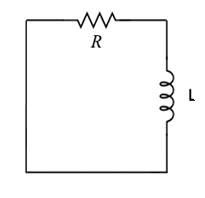
\includegraphics[width=0.33\textwidth]{images/Circuito_RL_4.png}
    }
    \subfloat[Intensidad nula.]{
        \label{fig::circuito_rl_4_2}
        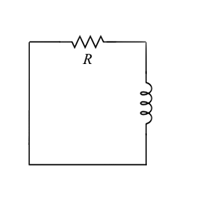
\includegraphics[width=0.33\textwidth]{images/Circuito_RL_5.png}
    }
    \caption{Disminución de corriente en un circuito RL.}
    \label{fig::carga_bobina_2}
\end{figure}


\subsubsection{Intensidad de corriente}
\label{part::descarga_inductor1}
Partiendo del balance energético planteado para el circuito RL en estado de disipación de energía
$$0 = V_L(t) + V_R(t)$$
obtenemos la siguiente ecuación diferencial, al aplicar \textit{Ley de Faraday-Lenz} y la \textit{Ley de Ohm} en la expresión anterior
$$0 = L\frac{d I(t)}{d t} + R \cdot I(t)$$
$$\frac{d I(t)}{I(t)} = -\frac{R}{L}d t $$
 
Suponiendo, que partimos de una posición dónde la intensidad de corriente es máxima (denotaremos por $I_0$ para simplificar), resolvemos la ecuación diferencial anterior utilizando el método de separación de variables. Integrando en ambos lados y resolviendo

$$\int_{I_0}^{I(t)} \frac{d I(t)}{I(t)} = \int_0^{t} -\frac{R}{L}d t $$
$$\Bigl[ \ln{I(t)} \Bigr]_{I_0}^{I(t)} = \frac{-R}{L} \left[ t \right]_0^{t}$$
$$\ln{I(t)} - \ln{I_0} = -\frac{R}{L}t$$
Si despejamos el término $I(t)$ de la expresión anterior, obtendremos la siguiente ecuación que modela la intensidad de corriente en el circuito (sabiendo que $I_0 = \frac{\varepsilon}{R}$):

\begin{equation}
    I(t) = \frac{\varepsilon}{R} \cdot e^{-Rt/L} 
\end{equation}



\subsubsection{Diferencia de potencial en la resistencia}
\label{part::descarga_inductor_2}
Usando la \textit{Ley de Ohm}, y la expresion que modela la intensidad de corriente en estado de disipación de energía, obtenemos que

\begin{equation}
    V_R(t) = \varepsilon \cdot e^{-Rt/L}
\end{equation}


\subsubsection{Diferencia de potencial en la bobina}
\label{part::descarga_inductor_3}
Por otro lado, para hallar la diferencia de potencial en el inductor, hacemos uso de la \textit{Ley de Faraday-Lenz}. Puesto que el signo nos indica el sentido de la corriente, podemos ignorarlo. La ecuación que modela este parámetro del circuito es:

\begin{equation}
    V_L(t) = -\varepsilon \cdot e^{-Rt/L}
\end{equation}


\subsection{Energía almacenada}
\label{part::energía_inductor}
Para hallar la energía que almacena un condensador, utilizaremos la definición de potencia almacenada en el inductor, usando para ello, la \textit{diferencia de potencial} en este dispositivo así como la intensidad de corriente eléctrica del circuito.
$$p(t) = V_L(t) \cdot I(t)$$
que esta \textit{ddp} puede reescribirse como
$$V_L(t) = L \frac{d I(t)}{d t}$$
, luego
$$p(t) = L \frac{d I(t)}{d t} I(t)$$
Sabiendo que, la energía consumida se expresa como
$$d E(t) = p(t) d t$$
Tenemos que
$$d E(t) = L I(t) d I(t)$$
Integramos a ambos lados, tomando como instante inicial un circuito donde la corriente eléctrica que atraviesa sus componentes es nula y, por consiguiente, la energía almacenada en el inductor también lo es
$$\int_0^{E(t)} d E(t) = \int_0^{I(t)} L I(t) d I(t)$$
$$E(t) = L \left[ \frac{I(t)^2}{2}\right]_0^{I(t)}$$
Siendo la expresión que modela la energía almacenada en la bobina

\begin{equation}
    E(t) = \frac{1}{2}L I(t)^2
\end{equation}



\subsection{Flujo magnético}
\label{part::flujo_magnetico_inductor}
Para obtener un modelo que exprese el \textit{flujo magnético} el función del tiempo, hacemos uso de la \textit{Ley de Faraday-Lenz} . 

$$d \phi(t) = L d I(t)$$

Partimos de igual manera de un circuito por el que no circula corriente eléctrica, así que resolvemos la ecuación diferencial anterior integrando a ambos lados, resultando que, la ecuación que modela el comportamiento del flujo magnético del inductor es:

\begin{equation}
    \phi(t) = L \cdot I(t)
\end{equation}


\end{document}